\documentclass{article}
\usepackage[utf8]{inputenc}
\usepackage{amsmath}
\usepackage{amsthm}
\usepackage[left=1in,right=1in,top=0.9in,bottom=0.9in]{geometry}
\usepackage{graphicx}
\usepackage{float}
\usepackage{titling}
\usepackage{algorithm}
\usepackage[noend]{algpseudocode}
\setlength{\droptitle}{-1.5cm}
\setlength\parindent{0pt}

\makeatletter
\def\BState{\State\hskip-\ALG@thistlm}
\makeatother


\title{Homework Report}
\date{Last modified: \today}
\author{Shawn Seymour\\ University of Minnesota Morris}

\newtheorem{prop}{Proposition}
\newtheorem*{theorem}{Theorem}

\theoremstyle{definition}
\newtheorem*{definition}{Definition}



\begin{document}

\maketitle

\section*{Vertex Coloring}
The vertex coloring problem (VCP) is one of the most common and most researched problems in graph theory. Vertex coloring is an assignment of colors, or labels, to each vertex in a graph \(G = (V, E)\) such that no edge connects two vertices of the same color. The vertex coloring problem aims to find the chromatic number of a graph, denoted \(\chi(G)\), the minimum number of colors needed to properly color a graph as defined above. The \emph{k-Colorability} problem asks where a graph can be colored with \(k\) colors.

\begin{prop}
Vertex coloring is a NP-hard problem.
\end{prop}

Coloring a graph is computationally complex. It is NP-hard to compute the chromatic number of a given graph \cite{garey}. 

\begin{prop}
The k-Colorability problem, i.e. can a given graph be colored in k-colors, is a NP-complete problem.
\end{prop}

To prove this, we need to reduce a known NP-complete problem to our coloring problem in polynomial time. By reducing a known NP-complete problem to k-Colorability, we can conclude that k-Colorability is NP-complete as all NP-complete problems are redicible to all other NP-complete problems \cite{gareynp}. We will reduce the well-known 3-SAT problem first to the 3-Colorability problem, and then from there reduce to the k-Colorability problem.

\subsection*{3-Satisfiability (3-SAT)}
The 3-SAT problem is an NP-complete problem that is a reduction of the original NP-complete problem, satisfiability (SAT). The 3-SAT problem is defined and proven to be NP-complete in \cite{gareynp}. 3-SAT consists of a conjunction of a number of clauses. A clause is a disjunction of a given number of propositions or their negations. We will assume all of our satisfiability problems are in conjunctive normal form (CNF). 3-SAT asks whether the variables can be assigned \emph{true} or \emph{false} in such a way that the whole expression evaluates to \emph{true}.

\begin{definition}
SAT is a conjunction of $m$ clauses, i.e. $C_1 \wedge C_2 \wedge \dots \wedge C_m$. Each clause is a disjunction of at most $n$ literals, i.e. $L_1 \vee L_2 \vee \dots \vee L_n$. Each literal can be a variable or negative of a variable, i.e. $x_1, \neg x_1, x_2, \neg x_2, \dots , x_k, \neg x_k$ where $k$ is the number of distinct literals. Each literal has a value of $true$ or $false$. 3-SAT is where each clause has exactly 3 literals \((n = 3)\).
\end{definition}

\subsection*{Reducing 3-SAT to 3-Colorability}
3-Colorability is NP-complete and was proven by \cite{moret}. To show this reduction, we need to:

\begin{enumerate}
\item Given an instance of 3-SAT, construct an instance of 3-Colorability
\item Show that the graph is 3-colorable, then the given 3-SAT problem is satisfied
\end{enumerate}

To show how this reduction can be done, I'll create an example 3-SAT problem and reduce it to 3-Colorability. Let's take the following 3-SAT expression:

\begin{align*}
\left( x_1 \vee \neg x_2 \vee \neg x_3 \right) \wedge \left( \neg x_1 \vee x_2 \vee x_3 \right) \wedge \left( x_1 \vee x_2 \vee x_3 \right)
\end{align*}


\section*{Heuristics}
As shown above, solving the VCP is very computationally heavy. There are heuristics that give a good, but not necessarily optimal, coloring of a given graph in polynomial time. I will be analyzing and comparing a few of the popular heuristics for solving the VCP. The input for all heuristics defined here is a simple graph \(G = (V, E)\). I will define them as follows:

\subsection*{Heuristic A}

Heuristic A is the greedy algorithm.

\begin{algorithm}
\caption{Greedy algorithm}
\begin{algorithmic}[1]
\State Label each vertex in $V$, i.e. $v_1, v_2, \dots, v_n$
\For{each $v \in V$}
\State Assign a color $p_i$ to $v_i$ using the smallest available $p_i$
\EndFor
\end{algorithmic}
\end{algorithm}

\subsection*{Heuristic B}

Heuristic B is the greedy algorithm with degree sequencing. It orders the vertices according to the decreasing value of their degree. This is also known as the Welsh-Powell algorithm, which is defined in \cite{welsh}.

\begin{algorithm}
\caption{Welsh-Powell algorithm}
\begin{algorithmic}[1]
\State Label each vertex in $V$, i.e. $v_1, v_2, \dots, v_n$, such that $d_G(v_1) \geq d_G(v_2) \geq \dots \geq d_G(v_n)$
\ForAll{$v \in V$}
\State Assign a color $p_i$ to $v_i$ using the smallest available $p_i$
\EndFor
\end{algorithmic}
\end{algorithm}

\subsection*{Heuristic C}

Heuristic C colors a graph by finding maximal independent sets of \(G\).

\begin{algorithm}
\caption{Coloring via maximal independent set algorithm}
\begin{algorithmic}[1]
\While{$G$ is non-empty}
\State Find a maximal independent set of $G$, i.e. $S_i$
\State Color all vertices in $S_i$ with color $p$, where $p$ is the smallest color available
\State Let $G \leftarrow G[V \setminus S_i ] $
\EndWhile
\end{algorithmic}
\end{algorithm}

\newpage

\section*{Findings}

\begin{prop}
Heuristic A and Heuristic B do not always produce an optimal solution, i.e. they do not always produce a minimum coloring of a graph.
\end{prop}

I will show this for \emph{heuristic B}. It is trivial to show the same for \emph{heuristic A} as \emph{heuristic B} includes the same steps as \emph{heuristic A}. I will construct a simple graph, \(G = (V, E)\), such that:

\begin{align}
|V| &\geq 8 \\
\chi(G) &> \chi^{*}(G)
\end{align}

Let \(\chi\) refer to the coloring of \(G\) generated by \emph{heuristic B}. Let \(\chi^{*}\) be the optimal coloring of \(G\).

\subsection*{Example 1}
I constructed a simple graph, \(G = (V, E)\), such that \(\Delta(G) = 3\) and \(\delta(G) = 1\). I've let \(|V| = 8\) for this example.

\begin{figure}[H]
\centering
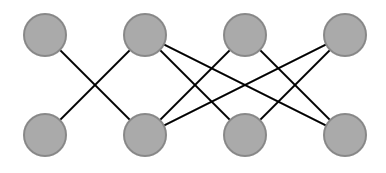
\includegraphics[scale=0.6]{images/graph-1.png}
\caption{Uncolored original graph \(G\)}
\end{figure}

By applying \emph{heuristic B}, we get the following coloring. The numbers indicate the ordering of vertices before applying the heuristic. Any vertex of the same degree got assigned arbitrarily. This results in \(\chi(G) = 3\).

\begin{figure}[H]
\centering
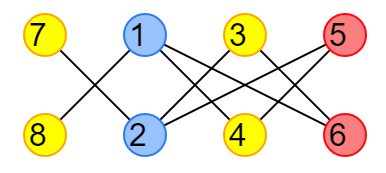
\includegraphics[scale=0.6]{images/graph-2.png}
\caption{Coloring from applying heuristic B}
\end{figure}

\begin{definition}[Bipartite graph]
A bipartite graph is one whose vertex set can be partitioned into two subsets X and Y such that each edge has one end in X and one end in Y
\end{definition}

We can see that this is a bipartite graph, defined above by \cite{bondymurty}. Thus, \(G\) is \emph{2-colorable}. This means \(\chi^{*}(G) = 2\). \(G\) is an example graph that satisfies conditions \((1)\) and \((2)\). The optimal coloring is shown below.

\begin{figure}[H]
\centering
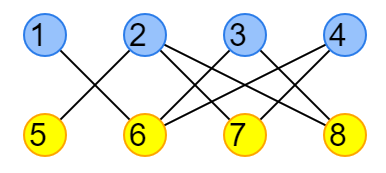
\includegraphics[scale=0.6]{images/graph-3.png}
\caption{Optimal coloring of graph \(G\)}
\end{figure}

\begin{prop}
Heuristic C also does not always produce an optimal solution, i.e. it does not always produce a minimum coloring of a graph.
\end{prop}

\subsection*{Example 2}
To show this, I will create another example that satisfies conditions \((1)\) and \((2)\) from above. I've constructed a graph \(K = (V,E)\) for this example.

\begin{figure}[H]
\centering
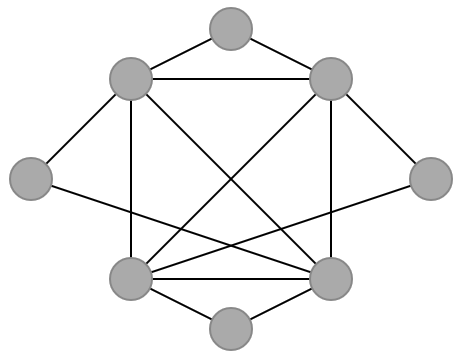
\includegraphics[scale=0.38]{images/mis-1.png}
\caption{Uncolored original graph \(K\)}
\end{figure}

By applying heuristic C and finding maximal independent sets, we see that \(K\) is \emph{5-colorable}.

\begin{figure}[H]
\centering
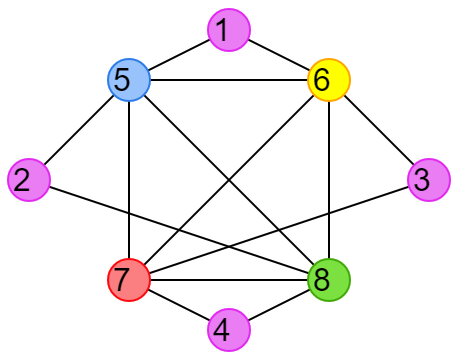
\includegraphics[scale=0.38]{images/mis-2.png}
\caption{Coloring of \(K\) after applying heuristic C}
\end{figure}

This is a non-optimal solution. We can see that the subgraph created by vertices \(\{5, 6, 7, 8\}\) is complete and thus we need at least 4 colors. This graph is \emph{4-colorable} however, meaning \(\chi^{*}(K) = 4\). Thus, we can see that heuristic C does not always give us an optimal solution.

\begin{figure}[H]
\centering
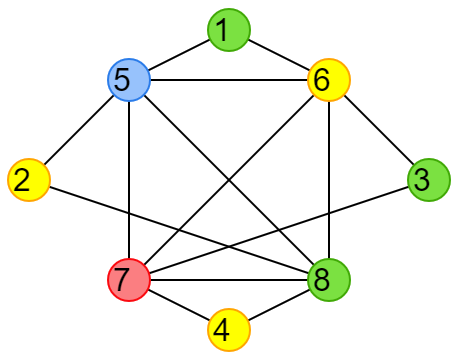
\includegraphics[scale=0.38]{images/mis-3.png}
\caption{Optimal coloring of \(K\)}
\end{figure}

\begin{prop}
Heuristic A and heuristic B have an upper bound of \(\Delta + 1\).
\end{prop}

To show this, I will create another example that satisfies conditions \((1)\) and \((2)\) from above. After doing some research into bipartite graphs, I learned that \emph{crown graphs} are excellent at showing how bad greedy heuristics can be, as shown and defined in \cite{kordecki}.

\begin{definition}[Crown Graph]
A crown graph \(CR_n = (V, E)\) is an undirected graph with two sets of vertices where \(V = V_1 \cup V_2\) with an edge from \(v_i \in V_1\) to \(v_{j} \in V_2\) whenever \(i \neq j\). A crown graph can also be viewed as a complete bipartite graph where the edges of a perfect matching have been removed.
\end{definition}

\subsection*{Example 3}

I constructed a simple crown graph, \(H = (V, E)\). I've let \(|V| = 10\) for this example.

\begin{figure}[H]
\centering
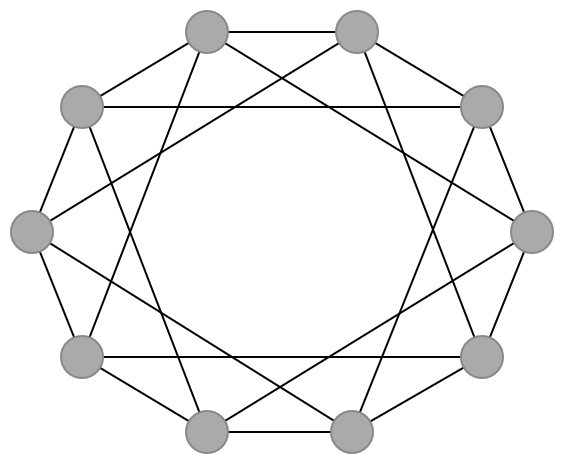
\includegraphics[scale=0.38]{images/graph-4.png}
\caption{Uncolored original graph \(H\)}
\end{figure}

We can see that \(\Delta(G) = 4\). We can also see \(d_G(v) = 4\) for all \(v \in V\). Thus, in both heuristics A and B, the greedy algorithm would pick an order arbitrarily. We can show using this crown graph the worst-case scenario of these heuristics.

\begin{figure}[H]
\centering
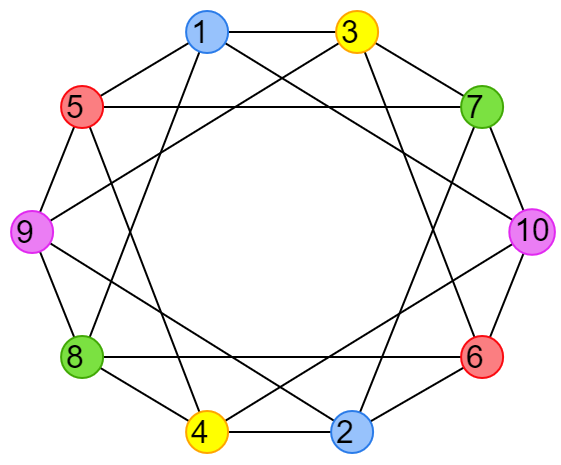
\includegraphics[scale=0.38]{images/graph-5.png}
\caption{Worst-case coloring of \(H\) using either heuristic A or B}
\end{figure}

In Figure 5, using either heuristic with this ordering, we get \(\chi(H) = 5\). This gives us \(\frac{|V|}{2}\) colors. This is the worst-case for a crown graph as shown in \cite{johnson}, but this graph also demonstrates the upper bounds for these heuristics. \newline

\textbf{In General}: Let's take a look at how this looks in general. Let \(P = (V, E)\) be a simple, complete graph. \newline

We can see that \(\chi(H) = \Delta(H) + 1\). This is very easy to see in a \emph{complete} graph, where all vertices are connected to every other vertex. This means all vertices have degree \(|V| - 1\). Thus, every time we color a node, a new color is needed. And since we have \(\Delta(P) = |V| - 1\) and \(|V|\) vertices, we will need \(\Delta(P) + 1\) colors. This is stated in \emph{Brooks' Theorem}.

\begin{theorem}[Brooks' Theorem]
For any connected undirected graph \(G\) with maximum degree \(\Delta\), the chromatic number of \(G\) is at most \(\Delta\) unless \(G\) is a complete graph or an odd cycle, in which case the chromatic number is \(\Delta + 1\).
\end{theorem}

The proof of \emph{Brook's Theorem} can be found in \cite{lovasz}. Overall, heuristic A and heuristic B can produce some very undesirable results. In graph \(H\), at the worst case, these heuristics produce \(\chi(H) = 5\) when \(\chi^{*}(H) = 2\) as it is bipartite. This is shown below.

\begin{figure}[H]
\centering
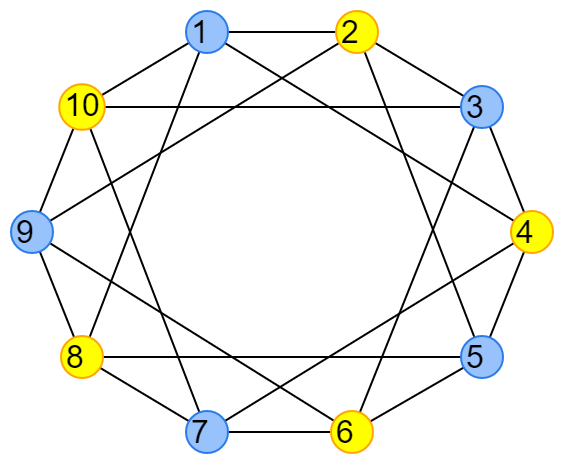
\includegraphics[scale=0.38]{images/graph-6.png}
\caption{Optimal coloring of \(H\)}
\end{figure}

\newpage

\begin{prop}
Heuristic A and Heuristic B have a running time of $O(|V| + |E|)$.
\end{prop}

It is possible to implement heuristic A and heuristic B efficiently and achieve a linear running time \cite{kubale}. By using an adjacency list representation of a graph \(G = (V, E)\), the greedy algorithm will look once at each vertex and each edge twice. This is because for each vertex, all of its neighbors are checked. This leads to the algorithm crossing each edge twuce. As this is still linear, we know \(O(|V| + 2|E|) = O(|V| + |E|)\).

\begin{prop}
Heuristic A and Heuristic B produce a feasible, proper coloring of input graph \(G = (V, E)\).
\end{prop}

Let \(G = (V, E)\) be a simple graph. Assume that two vertices, say \(v_1, v_2 \in V\), are connected by an edge \(e_1 \in E\). Assume that \(v_1, v_2\) are colored the same color, say \(p_1\). We know that in both heuristics, we assign the smallest color \(p_i\) that is not being used by any of the neighboring vertices connected by an edge \(e_i\). WLOG, the heuristic would color \(v_1\) color \(p_1\). The next iteration, while vertex \(v_2\) is selected, the heuristic would see color \(p_1\) is assigned to a neighboring vertex \((v_1)\), and assign the next available color \(p_2\). Thus, we've reached a contradiction.



\begin{thebibliography}{9}
\bibitem{bondymurty}
Bondy, J.A. and U.S.R. Murty [1976],
\emph{Graph theory with applications},
American Elsevier Publishing, New York, NY.

\bibitem{johnson}
Johnson, D. S. [1974], \emph{Worst-case behavior of graph coloring algorithms}, Proc. 5th Southeastern Conf. on Combinatorics, Graph Theory, and Computing, Utilitas Mathematicae, Winnipeg, pp. 513–527.

\bibitem{garey}
Garey, M. R., Johnson, D. S., and Stockmeyer, L. [1976], \emph{Some simplified NP-complete graph problems}, Theoretical computer science, 1(3), 237-267.

\bibitem{gareynp}
Garey, M.R. and Johnson, D.S. [2002], \emph{Computers and intractability} (Vol. 29), New York: wh freeman.

\bibitem{kordecki}
Kordecki, W. and A. Łyczkowska-Hanćkowiak [2016], \emph{Greedy online colouring with buffering}, arXiv preprint arXiv:1601.00252.

\bibitem{kubale}
Kubale, Marek [2004], \emph{Graph colorings}, Vol. 352, American Mathematical Soc.

\bibitem{lovasz}
Lovász, L. [1975], \emph{Three short proofs in graph theory}, Journal of Combinatorial Theory, Series B, 19(3), 269-271.

\bibitem{moret}
Moret, B.M. [1998], \emph{The theory of computation}, Addison-Wesley, Reading, Mass.

\bibitem{sharma}
Sharma, P. C. and Chaudhari, N.S. [2012], \emph{A new reduction from 3-SAT to graph k-colorability for frequency assignment problem}, Int. J. Comp. Applic, 23-27.

\bibitem{welsh}
Welsh, D. J. and Powell, M. B. [1967], \emph{An upper bound for the chromatic number of a graph and its application to timetabling problems}, The Computer Journal, 10(1), 85-86.

\end{thebibliography}


\end{document}
